
% This LaTeX was auto-generated from MATLAB code.
% To make changes, update the MATLAB code and republish this document.

\documentclass{article}
\usepackage{graphicx}
\usepackage{color}

\sloppy
\definecolor{lightgray}{gray}{0.5}
\setlength{\parindent}{0pt}

\begin{document}

    
    \begin{verbatim}
J = 0.1;
c = 6;
k = 343.77;
sys = tf(24,[J,c,k])
step(sys)

ylabel('\theta [rad]')
title('Q7.18 Step Response')
\end{verbatim}

        \color{lightgray} \begin{verbatim}
sys =
 
           24
  ---------------------
  0.1 s^2 + 6 s + 343.8
 
Continuous-time transfer function.

\end{verbatim} \color{black}
    
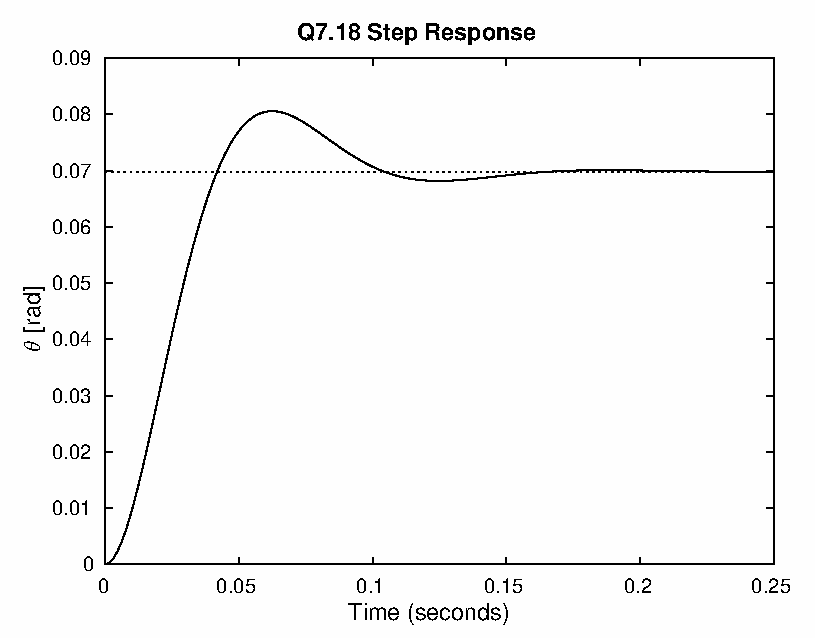
\includegraphics [width=4in]{Q7_18_01.eps}



\end{document}
    
